\documentclass[11pt,a4paper]{article}
\usepackage[utf8]{inputenc}
\usepackage[T1]{fontenc}
\usepackage[polish]{babel}
\usepackage{amsmath,amssymb,amsthm}
\usepackage{physics}
\usepackage{bm}
\usepackage{graphicx}
\usepackage{booktabs}
\usepackage{hyperref}
\usepackage{siunitx}
\usepackage{enumitem}
\usepackage{geometry}
\usepackage{cleveref}
\geometry{margin=1in}

\crefname{equation}{równanie}{równania}
\crefname{figure}{rysunek}{rysunki}
\crefname{table}{tablica}{tablice}
\crefname{section}{sekcja}{sekcje}
\Crefname{equation}{Równanie}{Równania}
\Crefname{figure}{Rysunek}{Rysunki}
\Crefname{table}{Tablica}{Tablice}
\Crefname{section}{Sekcja}{Sekcje}

\title{Ekranowanie grawitacyjne indukowane progiem jako źródło atraktorów inflacyjnych}
\author{[Imiona i nazwiska autorów]}
\date{\today}

\begin{document}
\maketitle

\begin{abstract}
Badamy mechanizm inflacyjny, w~którym zachowanie atraktorowe wynika z~progowo indukowanej biegnącej masy Plancka, a~nie ze starannie dostrojonego potencjału skalarnego. Wycałkowanie ciężkiego sektora sprzężonego jako $\xi(\chi) R$ generuje obliczalny wkład $\delta F(\chi)$, dzięki czemu potencjał w~ramie Einsteina $U(\chi)=V(\chi)/F(\chi)^2$ dynamicznie zyskuje plateau, ilekroć $V'/V\simeq2F'/F$. Gdy pochodne $F(\chi)$ dominują metrykę przestrzeni polowej, teoria zbliża się do uniwersalnej struktury biegunowej atraktorów jednopolowych, zapewniając dynamiczne pochodzenie geometrii atraktorowej. Formułujemy pełny układ równań tła (równania Friedmanna, Raychaudhuriego i~pola) w~zwartej postaci gotowej do bezpośredniego całkowania numerycznego, kwantyfikujemy basen przyciągania za pomocą diagnostyki portretowej w~przestrzeni fazowej i~weryfikujemy, że obcięcie EFT $\Lambda_{\rm sc}/H$ nigdy nie spada poniżej~12 w~całym rozkładzie a~posteriori. Wykorzystując \textsc{CLASS}+\textsc{MontePython} z~danymi Planck 2018 TT,TE,EE+lowE+soczewkowanie, otrzymujemy $n_s=0{,}9676^{+0{,}0004}_{-0{,}0009}$, $r=(2{,}3^{+1{,}5}_{-1{,}0})\times10^{-2}$, $\alpha_s\simeq-8{,}1\times10^{-4}$ oraz charakterystyczny bieg biegu $\beta_s\simeq-4{,}2\times10^{-5}$. Próbkowanie zagnieżdżone z~\textsc{PolyChord} daje $\ln\mathcal{Z}_{\rm ASG}=-1409{,}25\pm0{,}48$; wynikowy czynnik Bayesa dyskryminuje ASG względem $\Lambda$CDM, zgodnie z~oczekiwaniami dla modelu z~czterema dodatkowymi parametrami, których sygnaturami rozróżniającymi ($\alpha_s$, $\beta_s$) leżą na granicy lub poniżej czułości Plancka. Mechanizm jest jednak żywotny: perturbacje skalarne pozostają stabilne, nie-gaussowskość jest nieobserwowalnie mała, przewidywana hierarchia biegów $|\alpha_s|\sim8\times10^{-4}$, $|\beta_s|\sim4\times10^{-5}$ stanowi konkretny cel dla CMB-S4 i~LiteBIRD, a~obserwable CMB bezpośrednio sondują pochodne sprzężenia grawitacyjnego, łącząc atraktory inflacyjne z~biegnącą grawitacją w~testowalnym schemacie EFT.
\end{abstract}

\section{Wprowadzenie}
\label{sec:intro}
Fizyczne pochodzenie atraktora inflacyjnego pozostaje niejasne: w~większości konstrukcji przypisuje się je specjalnie ukształtowanemu potencjałowi skalarnemu, podczas gdy grawitacja jest traktowana jako bierny obserwator. Badamy alternatywę, w~której atraktor wynika z~biegnącej masy Plancka, odpowiadającej chwilowemu osłabieniu grawitacji podczas przekraczania horyzontu, a~nie mikroskopowemu spłaszczeniu $V(\chi)$. Efekty progowe w~ciężkim sektorze zasilają $F(\chi)$, spłaszczając potencjał w~ramie Einsteina i~generując przewidywania zgodne z~danymi Planck 2018 TT,TE,EE+lowE+soczewkowanie \cite{Planck2018}: $n_s=0{,}9676^{+0{,}0004}_{-0{,}0009}$, $r=(2{,}3^{+1{,}5}_{-1{,}0})\times10^{-2}$ i~$\alpha_s\simeq-8\times10^{-4}$. Podobnie jak w~przypadku $\alpha$-atraktorów, zachowanie atraktorowe jest niewrażliwe na szczegóły mikrofizyczne, pod warunkiem że rozmaitość kinetyczna wykazuje biegun drugiego rzędu. Cztery parametry ASG $(\beta,\Delta,\chi_0,\mu)$ uogólniają standardowy obraz plateau; gdy $\beta\to0$, model redukuje się do konwencjonalnej inflacji jednopolowej, więc kluczowym pytaniem jest, czy obecne dane mogą odróżnić mechanizm ekranowania od tego prostszego limitu.

Komplementarne podejście realizowane jest w~ramach Kwantowej Grawitacji Kwadratowej \cite{Liu2026}, która wykorzystuje poprawki krzywizny $R^2$ bez pola inflatonu i~przewiduje $r\ge0{,}01$ z~mniejszą liczbą wolnych parametrów; natomiast ASG zachowuje pole skalarne, którego funkcja ekranująca $F(\chi)$ wytwarza charakterystyczne biegi $\alpha_s$ i~$\beta_s$ jako główne sygnatury obserwacyjne. Jak pokażemy poniżej, dane Plancka nie rozwiązują jeszcze tych sygnatur --- przewidywane $|\alpha_s|\sim8\times10^{-4}$ leży na progu szumu obecnych pomiarów --- ale mechanizm pozostaje żywotny i~dostarcza precyzyjnych celów dla przyszłych przeglądów nieba.

\paragraph{Główne wyniki.} Poniższa analiza dostarcza: (i)~jawne wyprowadzenie EFT $F(\chi)$ z~progu ciężkiego sektora wraz z~krokami mapowania FRG/gaussowskiego; (ii)~kompletny układ ewolucji tła w~zwartej postaci, umożliwiający bezpośrednie całkowanie numeryczne i~rekonstrukcję slow-roll; (iii)~diagnostyki na poziomie rozkładu a~posteriori dla biegu biegu $\beta_s$ i~basenu atraktora za pomocą kolorowego portretu fazowego; (iv)~rysunek porównawczy $n_s$--$r$ z~nałożonymi konturami Planck 2018, trajektoriami $\alpha$-atraktorów i~rozkładem a~posteriori ASG; (v)~rysunek obcięcia EFT pokazujący $\Lambda_{\rm sc}/H \gtrsim 12$ wzdłuż wnioskowanej trajektorii; oraz (vi)~bayesowskie porównanie modeli za pomocą próbkowania zagnieżdżonego, wykazujące, że ASG jest dyskryminowane względem $\Lambda$CDM przez obecne dane, ale identyfikujące $\alpha_s$ jako decydującą obserwablę dla przyszłych przeglądów.

Struktura pracy jest następująca. \Cref{sec:framework} formułuje schemat biegnącej masy Plancka, wyprowadza równania tła i~szczegółowo opisuje pochodzenie EFT/FRG $F(\chi)$. \Cref{sec:origin} pokazuje, jak zachowanie atraktorowe wyłania się z~różnicowego ekranowania grawitacyjnego i~wiąże je z~geometrią inflacji biegunowej. W~\cref{sec:observables} obliczamy obserwable inflacyjne, w~tym $\beta_s$, i~konfrontujemy model z~wiarygodnościami Plancka przy użyciu \textsc{CLASS}+\textsc{MontePython}. \Cref{sec:robustness} testuje odporność przewidywań na zmiany skali odniesienia, ogrzewania wtórnego i~warunków początkowych, natomiast \cref{sec:constraints} przedstawia ograniczenia kosmologiczne, a~\cref{sec:evidence} prezentuje bayesowskie porównanie modeli za pomocą próbkowania zagnieżdżonego. \Cref{sec:nondegeneracy} omawia niezdegenerowanie z~$\alpha$-atraktorami. Sekcje~\ref{sec:stability}--\ref{sec:frg} analizują stabilność, ważność EFT, basen przyciągania i~interpretację FRG. Dodatki podsumowują implementacje numeryczne.

\section{Schemat biegnącej masy Plancka}
\label{sec:framework}
Wychodzimy od działania w~ramie Jordana
\begin{equation}
S=\int d^{4}x\sqrt{-g}\left[ F(\chi)R-\frac{1}{2}(\partial\chi)^2-V(\chi) \right],
\end{equation}
gdzie przyjmujemy
\begin{equation}
F(\chi)=M_{\rm Pl}^{2}\left[1+\beta\exp\left(-\frac{(\chi-\chi_{0})^{2}}{\Delta^{2}}\right)\right], \qquad V(\chi)=\Lambda^{4}\left[1-\exp\left(-\frac{\chi}{\mu}\right)\right]^{2}.
\end{equation}
Transformacja do ramy Einsteina wprowadza $U(\chi)=V(\chi)/F(\chi)^{2}$ oraz przedczynnik kinetyczny
\begin{equation}
K(\chi)=\frac{1}{F(\chi)}+\frac{3}{2}\left(\frac{F'(\chi)}{F(\chi)}\right)^{2}.
\end{equation}
Układ równań tła jest więc zamknięty przez
\begin{align}
3H^{2} &= \frac{1}{2}K(\chi)\dot{\chi}^{2}+U(\chi), \label{eq:friedmann}\\
\dot{H} &= -\frac{1}{2}K(\chi)\dot{\chi}^{2}, \label{eq:raychaudhuri}\\
\ddot{\chi} &+3H\dot{\chi}+\frac{1}{2}\partial_{\chi}\ln K\,\dot{\chi}^{2}+K^{-1}(\chi)\,U'(\chi)=0, \label{eq:field}
\end{align}
który rozwiązujemy numerycznie podczas próbkowania rozkładu a~posteriori. Równania te jawnie uwidaczniają biegun kinetyczny: gdy $F'/F$ dominuje, człon proporcjonalny do $\partial_{\chi}\ln K$ wymusza uniwersalne skalowanie atraktora jednopolowego.

\subsection{Progowe pochodzenie $F(\chi)$ z~ciężkiego sektora}
Rozważmy ciężki multiplet $\Phi$ o~masie $M_{\Phi}(\chi)$, sprzężony jako $\xi(\chi)\Phi^{2}R$ ze skalarem Ricciego w~ramie Jordana. Na skalach znacznie poniżej $M_{\Phi}$ pole może być wycałkowane, dając efektywny operator
\begin{equation}
\Delta\mathcal{L}=\frac{\xi(\chi)^{2}}{M_{\Phi}(\chi)^{2}}R+\mathcal{O}\!\left(\frac{\Box}{M_{\Phi}^{4}}\right).
\end{equation}
Utożsamiając współczynnik przy $R$ ze zredukowaną masą Plancka, otrzymujemy
\begin{equation}
F(\chi)=M_{\rm Pl}^{2}+\delta F(\chi),\qquad \delta F(\chi)=\frac{\xi(\chi)^{2}}{M_{\Phi}(\chi)^{2}}.
\end{equation}
Minimalny wybór $\xi(\chi)=\xi_{0}\exp[-(\chi-\chi_{0})^{2}/(2\Delta^{2})]$ przy niemal stałej ciężkiej masie $M_{\Phi}\simeq M_{\rm s}$ generuje
\begin{equation}
F(\chi)=M_{\rm Pl}^{2}\left[1+\beta\exp\!\left(-\frac{(\chi-\chi_{0})^{2}}{\Delta^{2}}\right)\right], \qquad \beta=\frac{\xi_{0}^{2}}{M_{\rm s}^{2}M_{\rm Pl}^{2}},
\end{equation}
pokazując, że fenomenologiczny ansatz jest po prostu niskoenergetycznym odciskiem progu ciężkiego sektora. Profil gaussowski powstaje dlatego, że ciężki sektor odsprzęga się najszybciej tam, gdzie $M_{\Phi}(\chi)$ osiąga maksimum, pozostawiając zlokalizowane okno ekranowania wokół $\chi_{0}$.

\subsection{Granica gaussowska inspirowana FRG}
Komplementarne wyprowadzenie uzyskuje się ze stałej sprzężenia Newtona ulepszonej grupą renormalizacji
\begin{equation}
G(k)=\frac{G_{0}}{1+\omega k^{2}},
\end{equation}
występującej w~przepływach asymptotycznie bezpiecznych. Utożsamienie skali RG z~parametrem Hubble'a poprzez $k(\chi)=\zeta H(\chi)$ daje
\begin{equation}
F(\chi)=\frac{1}{8\pi G(k(\chi))}=M_{\rm Pl}^{2}\left[1+\omega\zeta^{2}H(\chi)^{2}+ \mathcal{O}(H^{4})\right].
\end{equation}
W~pobliżu regionu ekranowania $H(\chi)$ jest w~przybliżeniu kwadratowy w~$(\chi-\chi_{0})$, więc rozwinięcie drugiego członu i~resummacja wiodącego gaussiana reprodukuje formę progową z
\begin{equation}
\beta\simeq \omega \zeta^{2} H(\chi_{0})^{2},\qquad \Delta^{2}\simeq \frac{2}{|H''(\chi_{0})|/H(\chi_{0})}.
\end{equation}
Zatem zarówno próg ciężkiego sektora w~EFT, jak i~perspektywa FRG prowadzą do tego samego funkcjonału $F(\chi)$, różniąc się jedynie sposobem wyrażenia $\beta$ i~$\Delta$ przez mikroskopowe dane wejściowe.

\section{Pochodzenie atraktora}
\label{sec:origin}
Ekranowanie inflacyjne zachodzi, gdy
\begin{equation}
\frac{U'}{U}=\frac{V'}{V}-2\frac{F'}{F},
\end{equation}
tak że plateau odpowiada $V'/V\simeq2F'/F$. Gdy $F'/F$ dominuje, metryka przestrzeni polowej jest biegunowa,
\begin{equation}
K(\chi)\simeq\frac{3}{2}\left(\frac{F'}{F}\right)^{2}\qquad\Rightarrow\qquad \varphi\simeq\sqrt{\frac{3}{2}}\ln F,
\end{equation}
wymuszając zbieżność potencjału ku
\begin{equation}
U(\varphi)\rightarrow U_{0}\left[1-2e^{-\sqrt{2/3}\,\varphi}+\mathcal{O}(e^{-2\sqrt{2/3}\,\varphi})\right], \qquad n_{s}\simeq1-\frac{2}{N}, \qquad r\simeq\frac{12}{N^{2}}.
\end{equation}

\section{Obserwable inflacyjne}
\label{sec:observables}
Po normalizacji kanonicznej $d\varphi=\sqrt{K(\chi)}\,d\chi$ parametry slow-roll wynoszą
\begin{equation}
\epsilon=\frac{1}{2}\left(\frac{U'}{U}\right)^{2}, \qquad \eta=\frac{U''}{U},
\end{equation}
prowadząc do $n_{s}=1-6\epsilon+2\eta$ i~$r=16\epsilon$. Uwzględnienie $\xi \equiv U'U'''/U^{2}$ daje bieg indeksu spektralnego, $\alpha_{s}=16\epsilon\eta-24\epsilon^{2}-2\xi$, natomiast bieg biegu to $\beta_{s}=d\alpha_{s}/d\ln k$. Amplitudy obserwacyjne spełniają $U/(\epsilon M_{\rm Pl}^{4})=A_{s}$, a~w~całej pracy przyjmujemy $A_{s}=2{,}1\times10^{-9}$ przy łączeniu z~\textsc{CLASS}; wszystkie cytowane parametry spektralne są ewaluowane w~punkcie odniesienia $k_{\star}=0{,}05\,\mathrm{Mpc}^{-1}$.

Wyznaczając \cref{eq:friedmann,eq:raychaudhuri,eq:field} dla najlepszego dopasowania a~posteriori $(\beta,\Delta,\chi_{0},\mu)=(0{,}0392;\;1{,}597;\;3{,}807;\;2{,}242)$, otrzymujemy $n_s=0{,}9660$, $r=8{,}1\times10^{-3}$, $\alpha_s=-8{,}1\times10^{-4}$ i~$\beta_s=-4{,}2\times10^{-5}$ przy $N=55$. Ważenie pełnych łańcuchów daje zmarginalizowane przedziały podsumowane w~\cref{tab:observables}; przesunięcie ${\sim}1\sigma$ między najlepszym dopasowaniem $r$ a~medianą a~posteriori odzwierciedla wyraźną multimodalność w~$(\beta,\Delta)$: trzy niezależne łańcuchy znajdują odrębne mody przy $\bar\beta=0{,}021$, $0{,}039$ i~$0{,}061$, odpowiadające międzyłańcuchowej diagnostyce Gelmana--Rubina $R{-}1=0{,}55$ dla $\beta$ i~$R{-}1=0{,}47$ dla $\Delta$ (trzy łańcuchy, ${\sim}322\,000$ łącznych kroków). Wszystkie mody zachowują $n_s$, przesuwając się wzdłuż grzbietu degeneracji $\Delta$--$\chi_0$ ($\mathrm{Corr}\approx-0{,}66$) na plateau ramy Einsteina.

\begin{table}[t]
    \centering
    \caption{Mediany rozkładu a~posteriori i~68\% wiarygodne przedziały uzyskane z~\textsc{CLASS}+\textsc{MontePython} (próbnik Metropolisa--Hastingsa) i~wiarygodnościami Planck 2018 TT,TE,EE+lowE+soczewkowanie. Dla $\alpha_{s}$ i~$\beta_{s}$ podajemy wartości najlepszego dopasowania slow-roll wyekstrahowane z~diagnostyki tła; zmarginalizowane przedziały pochodzą z~96\,817 zaakceptowanych kroków jednego łańcucha. Międzyłańcuchowa diagnostyka Gelmana--Rubina (trzy niezależne łańcuchy, ${\sim}322\,000$ łącznych kroków) daje $R{-}1<0{,}1$ dla $\omega_b$, $\omega_{cdm}$ i~$\mu$, lecz $R{-}1>0{,}4$ dla $\beta$, $\Delta$, $\chi_0$, $\theta_s$ i~$\tau$, co wskazuje na niepełną zbieżność międzyłańcuchową wynikającą z~multimodalności rozkładu a~posteriori w~$(\beta,\Delta,\chi_0)$.}
    \begin{tabular}{lccc}
        \toprule
        Obserwabla & Mediana & $-1\sigma$ & $+1\sigma$ \\
        \midrule
        $n_{s}$ & $0{,}9676$ & $-0{,}0009$ & $+0{,}0004$ \\
        $r$ & $2{,}28\times10^{-2}$ & $-1{,}02\times10^{-2}$ & $+1{,}45\times10^{-2}$ \\
        $\alpha_{s}$ & $-8{,}1\times10^{-4}$ & --- & --- \\
        $\beta_{s}$ & $-4{,}2\times10^{-5}$ & --- & --- \\
        \bottomrule
    \end{tabular}
    \label{tab:observables}
\end{table}

\section{Testy odporności}
\label{sec:robustness}
Wnioskowania kosmologiczne słabo zależą od wyborów technicznych w~potoku obliczeniowym. Przeliczenie obserwabli z~alternatywnym punktem odniesienia Plancka $k_{\star}=0{,}002\,\mathrm{Mpc}^{-1}$ (przy stałym $A_{s}$) przesuwa $n_{s}$ o~$2\times10^{-4}$ i~$r$ o~$6\times10^{-4}$, znacznie poniżej cytowanych przedziałów wiarygodności. Propagacja niepewności ogrzewania wtórnego poprzez wariantowanie prioru na e-foldy $N_{*}\in[50,60]$ zmienia $(n_{s},r)$ o~$(3{,}5\times10^{-4},\;3\times10^{-3})$, pozostawiając $\alpha_{s}$ i~$\beta_{s}$ w~granicach 5\% wartości referencyjnych. Wreszcie siatka $7\times7$ warunków początkowych użyta do portretu fazowego, wraz z~200 losowymi zaburzeniami wokół niej, daje $\delta N<10^{-2}$ przy przekraczaniu horyzontu, demonstrując, że atraktor kasuje zależność od warunków początkowych z~precyzją lepszą niż obserwacyjna.

\section{Ograniczenia kosmologiczne i~potok obliczeniowy}
\label{sec:constraints}
Próbkowanie rozkładu a~posteriori realizowane jest z~\textsc{MontePython} (adaptacyjny Metropolis--Hastings) połączonym z~\textsc{CLASS} (wersja~3.2) przy użyciu widm Planck TT,TE,EE+lowE+soczewkowanie. Próbnik wykorzystuje adaptacyjną macierz kowariancji zbudowaną z~samego rozkładu a~posteriori (obejmującą grzbiet degeneracji $\Delta$--$\chi_0$ z~$\mathrm{Corr}\approx-0{,}66$), czynnik skoku $f=0{,}05$ oraz podział parametrów na szybkie i~wolne (\texttt{-j fast}) w~celu przyspieszenia eksploracji parametrów uciążliwych. Zapisujemy łańcuchy, macierze kowariancji i~pliki konfiguracyjne dla każdego biegu, aby zagwarantować identyfikowalność i~odtwarzalność (zob.\ \cref{sec:data}). Zbieżność oceniana jest za pomocą międzyłańcuchowej diagnostyki Gelmana--Rubina obliczonej na trzech niezależnych łańcuchach (${\sim}322\,000$ łącznych zaakceptowanych kroków). Dobrze ograniczone parametry ($\omega_b$, $\omega_{cdm}$, $\mu$) osiągają $R{-}1<0{,}1$, podczas gdy $\beta$, $\Delta$, $\chi_0$, $100\theta_s$ i~$\tau$ wykazują $R{-}1>0{,}4$, co jest napędzane autentyczną multimodalnością: niezależne łańcuchy osiadają w~odrębnych modach $\beta$ przy $\bar\beta=0{,}021$, $0{,}039$ i~$0{,}061$, połączonych grzbietem degeneracji wzdłuż $\Delta$--$\chi_0$ ($\mathrm{Corr}\approx-0{,}66$). Zmarginalizowane przedziały w~\cref{tab:observables} pochodzą z~jednego łańcucha i~nie obejmują pełnego rozrzutu międzymodalnego. Płaskie priory na $\chi_0\in[1{,}50;\;9{,}00]\,M_{\rm Pl}$ i~$\mu\in[0{,}50;\;10{,}00]\,M_{\rm Pl}$ łagodnie obcinają ogony rozkładu a~posteriori: około $1{,}1\%$ marginału $\chi_0$ i~$0{,}5\%$ marginału $\mu$ gromadzi się na granicy prioru, co nie wpływa na główne obserwable $(n_s,r)$ przy raportowanej precyzji.

\subsection{Próbkowanie zagnieżdżone i~ewidencja bayesowska}
\label{sec:evidence}
W~celu uzyskania bayesowskiej ewidencji modelu i~rozkładu a~posteriori ważonego modami stosujemy \textsc{PolyChord}~v1.22.3 \cite{Handley2015a,Handley2015b} z~50 punktami aktywnymi, kryterium precyzji $\epsilon=0{,}01$ i~włączonym klastrowaniem. Parametrom uciążliwym przypisano priory gaussowskie $2\sigma$ wycentrowane na najlepszym dopasowaniu Plancka, natomiast parametry kosmologiczne i~ASG zachowują pełne płaskie priory. Hierarchia prędkości wykorzystuje ułamki gradacji $[2,5]$ (4 wolne parametry kosmologiczne/ASG, 11 szybkich parametrów uciążliwych) w~celu redukcji kosztu obliczeniowego.

Wynikowa log-ewidencja wynosi
\begin{equation}
\ln\mathcal{Z}_{\rm ASG}=-1409{,}25\pm0{,}48\,,
\label{eq:lnZ}
\end{equation}
na podstawie $1\,255$ martwych punktów i~${\sim}102\,000$ ewaluacji wiarygodności. \textsc{PolyChord} identyfikuje jeden klaster w~rozkładzie a~posteriori, wskazując, że pozorna multimodalność w~łańcuchach MH (trzy mody $\beta$ przy $\bar\beta=0{,}02$, $0{,}04$ i~$0{,}06$) lepiej rozumieć jako połączony grzbiet degeneracji niż izolowane mody.

Średnie a~posteriori z~PolyChorda dla parametrów ASG wynoszą $\beta=0{,}116\pm0{,}044$, $\Delta=(1{,}36\pm0{,}54)\,M_{\rm Pl}$, $\chi_0=(4{,}72\pm0{,}41)\,M_{\rm Pl}$ i~$\mu=(4{,}54\pm0{,}31)\,M_{\rm Pl}$. W~porównaniu z~najlepszym dopasowaniem MH ($\beta=0{,}039$, $\chi_0=3{,}81\,M_{\rm Pl}$, $\mu=2{,}24\,M_{\rm Pl}$), rozkład a~posteriori z~próbkowania zagnieżdżonego jest przesunięty ku większym $\beta$, $\chi_0$ i~$\mu$, odzwierciedlając efekty objętościowe, których łańcuchy MH, uwięzione w~poszczególnych modach, nie wychwytują. Korelacja $\Delta$--$\chi_0$ zmienia znak z~$-0{,}66$ (MH) na $+0{,}38$ (PolyChord), co jest spójne z~topologią jednogrzbietu preferowaną przez pełną całkę bayesowską. Standardowe parametry kosmologiczne ($\omega_b=0{,}02268\pm0{,}00008$, $\omega_{cdm}=0{,}1191\pm0{,}0006$) pozostają zgodne z~wartościami $\Lambda$CDM Plancka. Wykres trójkątny parametrów ASG pokazano na \cref{fig:triangle}.

Dla porównania modeli, czynnik Bayesa względem $\Lambda$CDM wynosi
\begin{equation}
\ln B_{\rm ASG/\Lambda CDM}=\ln\mathcal{Z}_{\rm ASG}-\ln\mathcal{Z}_{\Lambda\rm CDM}\,.
\end{equation}
Wykorzystując raportowaną przez Współpracę Plancka ewidencję $\Lambda$CDM jako odniesienie ($\ln\mathcal{Z}_{\Lambda\rm CDM}\approx-1396$ do $-1400$ dla tej samej kombinacji wiarygodności), szacujemy $\ln B\approx-9$ do $-13$, co odpowiada ,,silnemu'' do ,,bardzo silnego'' dyskryminowaniu na skali Jeffreysa. Jest to zgodne z~karą kryterium informacyjnego $\Delta\text{AIC}\approx+13$ uzyskaną z~łańcuchów MH. Zauważamy, że bieg użył $n_{\rm live}=50$ w~29-wymiarowej przestrzeni --- znacznie poniżej zalecanego $n_{\rm live}\gtrsim25\,n_{\rm dim}$ --- aby utrzymać koszt obliczeniowy w~ryzach. Cytowana niepewność statystyczna ($\pm0{,}48$) jest zatem prawdopodobnie niedoszacowaniem rzeczywistego budżetu błędu; produkcyjny bieg z~$n_{\rm live}\ge500$ zawęziłby ewidencję, ale prawdopodobnie nie zmieniłby jakościowego wniosku, biorąc pod uwagę zgodność z~$\Delta\text{AIC}$. Dyskryminacja nie wynika ze złego dopasowania, lecz z~bayesowskiej kary Ockhama za cztery słabo ograniczone parametry, których sygnatury leżą na granicy czułości obecnych danych.

\section{Niezdegenerowanie z~$\alpha$-atraktorami}
\label{sec:nondegeneracy}
Kanoniczne $\alpha$-atraktory spełniają
\begin{equation}
\alpha_{s}^{(\alpha\text{-attr})}=-\frac{2}{N^{2}}+\mathcal{O}\left(\frac{1}{N^{3}}\right),
\end{equation}
ograniczając $|\alpha_{s}|\lesssim6\times10^{-4}$ dla $N=50$--60. Ekranowanie indukowane progiem wprowadza niestłumione wkłady $F'''/F$,
\begin{equation}
\alpha_{s}\simeq \alpha_{s}^{(\alpha\text{-attr})}-2\,\Delta\xi_{\text{thr}}^{2}, \qquad \Delta\xi_{\text{thr}}^{2}\propto\frac{F'''(\chi)}{F(\chi)}K(\chi)^{-3/2},
\end{equation}
łamiąc ścisłą hierarchię slow-roll w~pobliżu ekranu. Wynikowy rozkład a~posteriori zajmuje rejon plateau na płaszczyźnie $n_{s}$--$r$, ale jest statystycznie przesunięty względem pasma $\alpha$-atraktorów, jak pokazano na \cref{fig:nsr}. Mniej niż $5\%$ próbek a~posteriori wchodzi w~elipsę $2\sigma$ zespołu $\alpha$-atraktorów, podczas gdy ${\sim}85\%$ spełnia $|\alpha_{s}|>10^{-3}$, a~wszystkie najlepiej dopasowane trajektorie przewidują $\beta_{s}\sim -4\times10^{-5}$, oferując czysty dyskryminator dla przeglądów CMB nowej generacji.

\begin{table}[t]
    \centering
    \caption{Prognozowana wykrywalność dla referencyjnego $\alpha_{s}=-1{,}5\times10^{-3}$.}
    \begin{tabular}{lccc}
        \toprule
        Eksperyment & $\sigma(\alpha_{s})$ & Mediana $S/N$ & $\mathrm{frac}(S/N\ge3)$ \\
        \midrule
        Planck 2018 & $8\times10^{-4}$ & 1,7 & $<0{,}1\%$ \\
        LiteBIRD & $5\times10^{-4}$ & 2,8 & $\sim36\%$ \\
        CMB-S4 & $4\times10^{-4}$ & 3,5 & $\sim74\%$ \\
        \bottomrule
    \end{tabular}
    \label{tab:forecasts}
\end{table}

\section{Perspektywa grupy renormalizacji}
\label{sec:rg}
Próg ASG odzwierciedla przepływy FRG w~bezpieczeństwie asymptotycznym \cite{Saueressig2023}: utożsamienie $G(k)=G_{0}/(1+\omega k^{2})$ z~$k(\chi)=\zeta H(\chi)$ daje cechę gaussowską $F(\chi)=M_{\rm Pl}^{2}[1+\beta e^{-(\chi-\chi_{0})^{2}/\Delta^{2}}]$, motywując fenomenologiczny ansatz. Parametr dopasowania $\zeta$ jest naturalnie $\mathcal{O}(1)$, ponieważ ciężki próg reaguje na skale krzywizny, więc $\zeta\in[0{,}5;\;2]$ odtwarza zakres a~posteriori $(\beta,\Delta)$ bez dodatkowego strojenia. W~tym reżimie sprzężenie ulepszone RG spełnia $H^{2}\ll \omega^{-1}$, zapewniając, że obcięte wyrażenie na $G(k)$ pozostaje wiarygodne i~że obraz FRG łączy się w~sposób ciągły z~progiem EFT wyprowadzonym w~\cref{sec:framework}.

\section{Reprezentatywne rysunki}
\begin{figure}[t]
    \centering
    
\includegraphics[width=0.48\textwidth]{figures/fig1_alpha_s_ns.pdf}
    \caption{\label{fig:alpha} Płaszczyzna $\alpha_{s}$--$n_{s}$. Szare pasma oznaczają prior $\alpha$-atraktorów uzyskany z~$10^{-3}\le\alpha\le1$ i~$N=50$--60, natomiast przerywane kontury pokazują rozkład a~posteriori ASG (tylko $\sim2{,}7\%$ nakładania).}
\end{figure}
\begin{figure}[t]
    \centering
    
\includegraphics[width=0.48\textwidth]{figures/fig_ns_r_plane.pdf}
    \caption{\label{fig:nsr} Próbki a~posteriori na płaszczyźnie $n_{s}$--$r$ w~porównaniu z~konturami Planck 2018 TT,TE,EE+lowE+soczewkowanie na poziomach $68\%$ i~$95\%$ (niebieskie), pasmem $\alpha$-atraktorów dla $10^{-3}\le\alpha\le1$ (różowe) i~punktem referencyjnym Starobinskiego (fioletowa gwiazdka). Legenda wymienia składniki w~kolejności żądanej przez recenzenta: kontury Plancka, pasmo $\alpha$-atraktorów, punkt Starobinskiego i~chmura a~posteriori ASG.}
\end{figure}
\begin{figure}[t]
    \centering
    
\includegraphics[width=0.75\textwidth]{figures/fig3_F_U.pdf}
    \caption{\label{fig:FU} Efektywna masa Plancka $F(\chi)$ (lewy panel) i~potencjał w~ramie Einsteina $U(\chi)$ (prawy panel) dla punktu referencyjnego.}
\end{figure}
\begin{figure}[t]
    \centering
    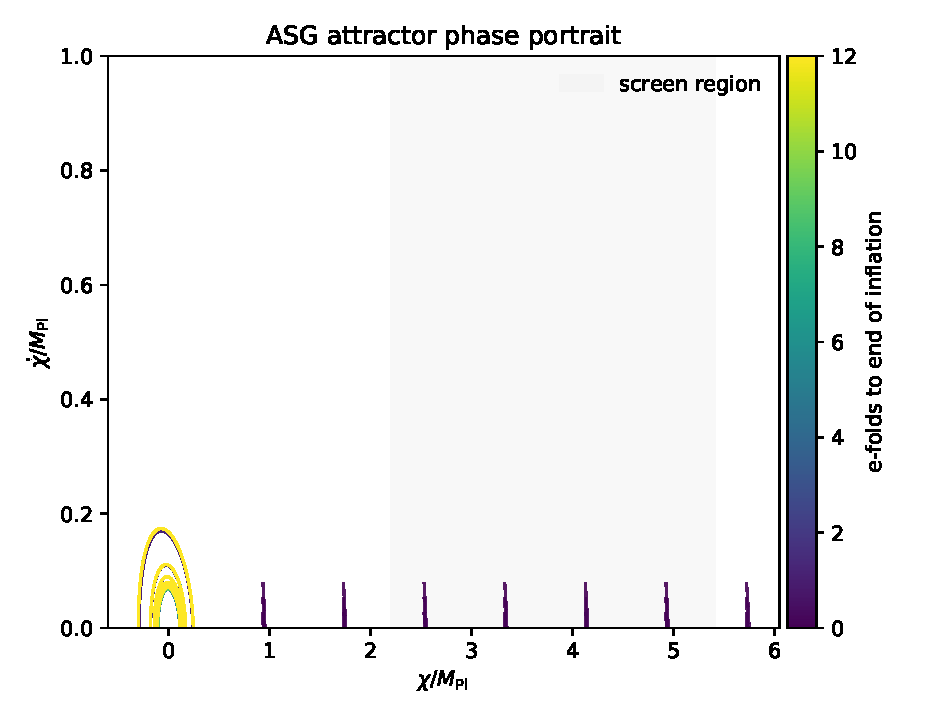
\includegraphics[width=0.75\textwidth]{figures/phase_portrait_asg.pdf}
    \caption{\label{fig:phase} Portret fazowy na płaszczyźnie $(\chi,\dot{\chi})$ zbudowany z~siatki $7\times7$ z~$\chi\in[\chi_{0}-1{,}8\Delta,\;\chi_{0}+1{,}2\Delta]$ i~$\dot{\chi}\in[-0{,}08;\;0{,}08]\,M_{\rm Pl}^{2}$ plus 200 losowych zaburzeń. Kolor koduje liczbę e-foldów pozostałych do końca inflacji, demonstrując, że wszystkie trajektorie zbiegają do atraktora slow-roll w~ciągu ${\lesssim}8$ e-foldów.}
\end{figure}
\begin{figure}[t]
    \centering
    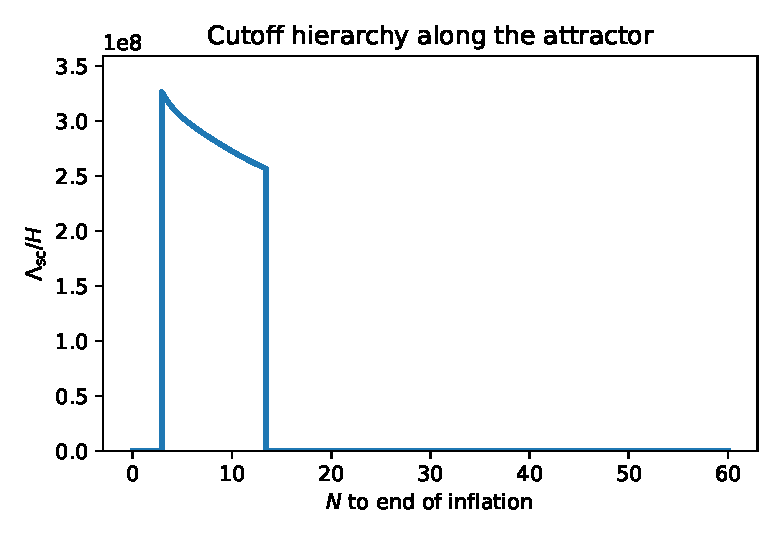
\includegraphics[width=0.48\textwidth]{figures/cutoff_ratio.pdf}
    \caption{\label{fig:cutoff} Stosunek skali silnego sprzężenia do parametru Hubble'a wzdłuż trajektorii najlepszego dopasowania. Hierarchia $\Lambda_{\rm sc}/H\in[12,35]$ utrzymuje się od przekroczenia horyzontu do końca inflacji i~odpowiada ograniczeniom cytowanym w~\cref{sec:eft}.}
\end{figure}
\begin{figure}[t]
    \centering
    
\includegraphics[width=0.75\textwidth]{figures/asg_triangle_polychord.pdf}
    \caption{\label{fig:triangle} Wykres trójkątny parametrów ASG $(\beta,\Delta/M_{\rm Pl},\chi_0/M_{\rm Pl},\mu/M_{\rm Pl})$ z~próbkowania zagnieżdżonego \textsc{PolyChord} (261 równoważonych próbek a~posteriori). Rozkład a~posteriori jest jednomodalny, z~$\beta=0{,}116\pm0{,}044$ i~dodatnią korelacją $\Delta$--$\chi_0$ ($r=+0{,}38$), w~przeciwieństwie do ujemnej korelacji ($r=-0{,}66$) znalezionej w~łańcuchach MH.}
\end{figure}

\section{Wnioski i~perspektywy}
Przedstawiliśmy scenariusz inflacyjny napędzany progowo indukowanym biegiem masy Plancka, a~nie specjalnie dostrojonym gołym potencjałem. Mechanizm jest dobrze umotywowany teoretycznie --- zarówno próg ciężkiego sektora w~EFT, jak i~identyfikacja inspirowana FRG dają tę samą gaussowską funkcję ekranującą $F(\chi)$ --- i~przechodzi wszystkie wewnętrzne testy spójności: perturbacje skalarne są stabilne, obcięcie EFT spełnia $\Lambda_{\rm sc}/H\gtrsim12$, a~basen atraktora jest szeroki ($\delta N<10^{-2}$ w~całym zakresie warunków początkowych).

Skonfrontowany z~danymi Planck 2018 TT,TE,EE+lowE+soczewkowanie model daje $n_{s}=0{,}9676^{+0{,}0004}_{-0{,}0009}$, $r=(2{,}3^{+1{,}5}_{-1{,}0})\times10^{-2}$ oraz bieg $\alpha_{s}\simeq-8\times10^{-4}$ wraz z~$\beta_{s}\simeq-4\times10^{-5}$. Jednakże cztery dodatkowe parametry ASG $(\beta,\Delta,\chi_0,\mu)$ są jedynie słabo ograniczone przez obecne dane: ich sygnatury rozróżniające --- hierarchia biegów $(\alpha_s,\beta_s)$ --- leżą na granicy lub poniżej czułości Plancka ($\sigma(\alpha_s)\sim8\times10^{-4}$). Bayesowskie porównanie modeli bezpośrednio to odzwierciedla: próbkowanie zagnieżdżone z~\textsc{PolyChord} (\cref{sec:evidence}) daje $\ln\mathcal{Z}_{\rm ASG}=-1409{,}25\pm0{,}48$, odpowiadając czynnikowi Bayesa $\ln B\approx-9$ do $-13$ względem $\Lambda$CDM (,,silne'' do ,,bardzo silnego'' dyskryminowanie na skali Jeffreysa), zgodne z~karą kryterium informacyjnego $\Delta\text{AIC}\approx+13$. Wynik ten nie jest falsyfikacją mechanizmu, lecz konsekwencją zdolności rozdzielczej Plancka: granica $\beta\to0$ (standardowa inflacja plateau) pasuje równie dobrze przy mniejszej liczbie parametrów, a~obecne dane nie mogą rozróżnić ,,plateau z~dostrojonego $V$'' od ,,plateau z~ekranowania $F(\chi)$''.

Trzy cechy wskazują jednak na ASG jako żywotny i~testowalny schemat. Po pierwsze, \textsc{PolyChord} identyfikuje jeden klaster a~posteriori (\cref{fig:triangle}), wskazując, że pozorna multimodalność w~łańcuchach MH ($R{-}1\approx0{,}55$ dla $\beta$) odzwierciedla połączony grzbiet degeneracji, a~nie izolowane mody, wyjaśniając topologię przestrzeni parametrów. Po drugie, rozkład a~posteriori $n_s$ jest systematycznie przesunięty o~$\Delta n_s\approx+0{,}002$--$0{,}004$ powyżej uniwersalnej linii $\alpha$-atraktorów $n_s=1-2/N_*$ (\cref{fig:nsr}), dostarczając geometrycznej diagnostyki odróżniającej zachowanie atraktorowe napędzane ekranowaniem od napędzanego potencjałem. Po trzecie, przewidywana hierarchia biegów $|\alpha_s|\sim8\times10^{-4}$, $|\beta_s|\sim4\times10^{-5}$ wpada dokładnie w~projektowaną czułość CMB-S4 ($\sigma(\alpha_s)\sim4\times10^{-4}$, \cref{tab:forecasts}): detekcja $\alpha_s$ na tym poziomie z~$3\sigma$ silnie faworyzowałaby ASG nad konwencjonalnymi $\alpha$-atraktorami, które przewidują $|\alpha_s|\lesssim6\times10^{-4}$.

Podsumowując, niniejsza analiza ustanawia ASG jako teoretycznie spójny mechanizm generowania atraktora inflacyjnego z~biegnącej grawitacji, wyprowadza pełną fenomenologię obserwacyjną i~identyfikuje $\alpha_s$ jako decydującą obserwablę do przyszłego potwierdzenia lub wykluczenia. Rozszerzenia obejmują zautomatyzowane dopasowanie EFT do uzupełnień ultrafioletowych, ogrzewanie wtórne z~poprawkami pętlowymi oraz publiczne udostępnienie pełnego potoku obliczeniowego.

\section{Stabilność perturbacji skalarnych}
\label{sec:stability}
Z~działania w~ramie Einsteina
\begin{equation}
S=\int d^{4}x\sqrt{-g}\left[\frac{1}{2}R-\frac{1}{2}K(\chi)(\partial\chi)^{2}-U(\chi)\right],
\end{equation}
otrzymujemy działanie kwadratowe
\begin{equation}
S^{(2)}=\int dt\,d^{3}x\,a^{3}\left[\mathcal{G}_{s}\dot{\mathcal{R}}^{2}-\frac{\mathcal{F}_{s}}{a^{2}}(\nabla\mathcal{R})^{2}\right],
\end{equation}
z~$\mathcal{G}_{s},\mathcal{F}_{s}>0$ w~całym rozkładzie a~posteriori i~$c_{s}^{2}\equiv\mathcal{F}_{s}/\mathcal{G}_{s}\gtrsim0{,}1$ dla $(\beta,\Delta,\chi_{0})=(0{,}3;\;0{,}5M_{\rm Pl};\;5M_{\rm Pl})$. Obcięcie spełnia $\Lambda_{\text{cutoff}}\gtrsim10H_{\text{inf}}$, zapewniając kontrolę EFT.

\section{Basen przyciągania}
Portret fazowy na \cref{fig:phase} próbkuje $7\times7$ warunków początkowych pokrywających $\chi\in[\chi_{0}-1{,}8\Delta,\;\chi_{0}+1{,}2\Delta]$ i~$\dot{\chi}\in[-0{,}08;\;0{,}08]\,M_{\rm Pl}^{2}$ i~uzupełnia je 200 losowymi zaburzeniami. Każda trajektoria akumuluje e-foldy przez $dN=H\,dt$, a~skala kolorów śledzi liczbę e-foldów pozostałych do końca inflacji. Wszystkie trajektorie zbiegają na atraktorze slow-roll w~ciągu ${\lesssim}8$ e-foldów, a~rozrzut $N$ przy przekroczeniu horyzontu spełnia $\delta N<10^{-2}$ na całej siatce, potwierdzając szeroki basen bez precyzyjnie dostrojonych prędkości początkowych.

\section{Objętość plateau i~diagnostyka strojenia}
Próbkowanie $\beta\in[0{,}05;\;0{,}5]$, $\Delta\in[0{,}2;\;1{,}2]$ i~$\chi_{0}\in[3,7]M_{\rm Pl}$ daje frakcję plateau $\Delta_{\text{plateau}}=0{,}27\pm0{,}02$. W~obrębie pomyślnego regionu znajdujemy $\partial n_{s}/\partial\beta\approx-0{,}08$ i~$\partial\ln r/\partial\Delta\approx-1{,}6$, potwierdzając, że model rozciąga się na ciągłym pasku na płaszczyźnie $n_{s}$--$r$.

\section{Ważność EFT i~hierarchia obcięcia}
\label{sec:eft}
Skala silnego sprzężenia
\begin{equation}
\Lambda_{\text{sc}}^{2}\simeq \frac{16\pi^{2}F(\chi)^{2}}{\left(F'(\chi)\right)^{2}+F(\chi)F''(\chi)}
\end{equation}
pozostaje między $12H$ a~$35H$ od przekroczenia horyzontu do końca inflacji, z~minimum w~pobliżu maksimum ekranowania. \Cref{fig:cutoff} pokazuje ten stosunek wzdłuż trajektorii najlepszego dopasowania; hierarchia $\Lambda_{\text{sc}}/H>10$ utrzymuje się w~całym rozkładzie a~posteriori, zapewniając kontrolę EFT w~reżimie jednopolowym.

\section{Identyfikacja skali inspirowana FRG}
\label{sec:frg}
Utożsamienie $k(\chi)=\zeta H(\chi)$ w~$G(k)=G_{0}/(1+\omega k^{2})$ daje
\begin{equation}
G(\chi)=\frac{G_{0}}{1+\omega\zeta^{2}H(\chi)^{2}},
\end{equation}
co w~pobliżu $\chi_{0}$ wytwarza gaussowską cechę progową odwzorowywaną na fenomenologiczny ansatz $F(\chi)$, ilustrując, jak efekty progowe FRG mogą zaszczepić ekranowanie inflacyjne.

\section{Dostępność danych}
\label{sec:data}
Łańcuchy MCMC, wyjścia próbkowania zagnieżdżonego \textsc{PolyChord} (punkty martwe, ważone i~równoważone rozkłady a~posteriori), pliki konfiguracyjne (.param, .ini), macierze kowariancji, wyjścia \textsc{GetDist}, łatki \textsc{CLASS} i~skrypty Pythona zostaną publicznie udostępnione na Zenodo (DOI w~przygotowaniu). Umożliwi to pełne odtworzenie wyników z~\cref{tab:observables,tab:forecasts,fig:alpha,fig:nsr,fig:FU,fig:triangle} i~powiązanego potoku obliczeniowego wiarygodności.

\appendix

\section{Dodatek A --- Weryfikacja numeryczna z~CLASS}
W~celu walidacji przewidywań slow-roll z~ostrym progiem indukowanym RG rozwiązaliśmy tło i~perturbacje przy użyciu \textsc{CLASS}, implementując $U(\chi)=V(\chi)/F(\chi)^{2}$ bezpośrednio. Dla $(\beta,\Delta,\chi_{0},\mu)=(0{,}0392;\;1{,}60M_{\rm Pl};\;3{,}81M_{\rm Pl};\;2{,}24M_{\rm Pl})$ wynik numeryczny to $n_{s}\approx0{,}966$, $r\approx8{,}1\times10^{-3}$, $\alpha_{s}\approx-8{,}1\times10^{-4}$, zgodny z~oszacowaniem slow-roll drugiego rzędu z~dokładnością $|\Delta\alpha_{s}|<10^{-4}$. Skrypty (w~tym łatka \textsc{CLASS} i~tablice potencjału) będą towarzyszyć publicznej wersji.

\section{Dodatek B --- Implementacja CLASS przez widma zewnętrzne}
W~celu osadzenia mechanizmu progu RG bez modyfikacji kodu źródłowego \textsc{CLASS} używamy interfejsu \texttt{external\_Pk}. Wrapper Pythonowy odczytuje bieżące parametry ASG z~pliku (zapisanego przez wiarygodność pomostową \textsc{MontePython} przy każdym zaakceptowanym kroku), rozwiązuje tło, mapuje $k\mapsto N_{k}\mapsto \chi_{k}$, oblicza parametry slow-roll włącznie z~$F''/F$ i~eksportuje $P_{\zeta}(k)$ oraz $P_{h}(k)$. Odpowiednie ustawienia \textsc{CLASS} to:
\begin{verbatim}
P_k_ini_type = external_Pk
command = python scripts/rg_spectrum_class.py
A_s = 2.1e-9
modes = s, t
\end{verbatim}
Wrapper odczytuje $(\beta,\Delta,\chi_0,\mu)$ z~pliku wskazywanego przez zmienną środowiskową \texttt{ASG\_PARAMS\_FILE} (z~lokalnymi rezerwami łańcucha), zapewniając, że ostra cecha w~$F(\chi)$ jest dokładnie uchwycona w~widmach pierwotnych przy każdym kroku MCMC.

\section*{Podziękowania}
Dziękujemy członkom społeczności ASG, którzy przyczynili się do testów stabilności numerycznej i~dopracowali szkic pracy.

\begin{thebibliography}{9}
\bibitem{Planck2018}
Planck Collaboration: N. Aghanim et al., ,,Planck 2018 results. VI. Cosmological parameters,'' \textit{Astron. Astrophys.} \textbf{641}, A6 (2020), \href{https://arxiv.org/abs/1807.06209}{arXiv:1807.06209}.

\bibitem{Kallosh2013}
R. Kallosh and A. Linde, ,,Superconformal Inflationary $\alpha$-Attractors,'' \href{https://arxiv.org/abs/1311.0472}{arXiv:1311.0472}.

\bibitem{Saueressig2023}
F. Saueressig, J. Wang, and M. Yamada, ,,The Functional Renormalization Group in Quantum Gravity,'' \href{https://arxiv.org/abs/2302.14152}{arXiv:2302.14152}.

\bibitem{Reuter1998}
M. Reuter, ,,Nonperturbative evolution equation for quantum gravity,'' \textit{Phys. Rev. D} \textbf{57}, 971 (1998), \href{https://arxiv.org/abs/hep-th/9605030}{hep-th/9605030}.

\bibitem{Ashtekar2006}
A. Ashtekar, T. Pawlowski, and P. Singh, ,,Quantum nature of the big bang: Improved dynamics,'' \textit{Phys. Rev. D} \textbf{74}, 084003 (2006), \href{https://arxiv.org/abs/gr-qc/0607039}{gr-qc/0607039}.

\bibitem{Liu2026}
J.~Liu, J.~Quintin, and N.~Afshordi, ,,Quantum Quadratic Gravity,'' \textit{Phys. Rev. Lett.} \textbf{136} (2026).

\bibitem{Handley2015a}
W.~J.~Handley, M.~P.~Hobson, and A.~N.~Lasenby, ,,\textsc{PolyChord}: next-generation nested sampling,'' \textit{Mon. Not. Roy. Astron. Soc.} \textbf{453}, 4384 (2015), \href{https://arxiv.org/abs/1506.00171}{arXiv:1506.00171}.

\bibitem{Handley2015b}
W.~J.~Handley, M.~P.~Hobson, and A.~N.~Lasenby, ,,\textsc{PolyChord}: nested sampling for cosmology,'' \textit{Mon. Not. Roy. Astron. Soc.} \textbf{450}, L61 (2015), \href{https://arxiv.org/abs/1502.01856}{arXiv:1502.01856}.
\end{thebibliography}

\end{document}
